%!TEX root = ../Thesis.tex
\chapter{An Appendix}


\section{Random forest Q and A answers with illustrations and code examples}

During the last three years, two forums \textit{Stack Overflow} \url{http://stackoverflow.com/} for learning programming and \textit{Cross Validated} \url{stats.stackexchange.com} for learning statistics have been invaluable daily sources of fast answers to questions on all levels. When getting stuck and that probably happens 10 times a day, one only have to complain to google search about the problem in a sentence. As we are six billions on this planet, odds are some person on the same level already had this problem before, and posed the same question in same silly wording as you do, and some kind person have already answered with a practical example, and perhaps also provided answers to some other question, one really ought to be asking instead. The cross validated site is relatively small with only 83,000 questions (July 2016), where \textit{Stack Overflow} has 12,000,000 questions as cover most programming languages. For the entertainment value and to test my knowledge on random forest, I started to answer questions my self. By putting my beliefs on public display, I sometimes receive swift criticism, when I'm wrong. I have answered 92 questions. Each answer takes in average  a page long and often comprises visulizations, coding, references to other material and takes hour to write. I will include some of my favorite answers here, and some time refer to these from other chapters. The site has almost 100.000 users, and reputation voting wise, I rank top 200. My answers have presently in total 70,000 page views (~50.000 views/yr), which is probably some 4 orders of magnitude more than this chapter will have.


\subsection{Handling unbalanced data with with random forest}
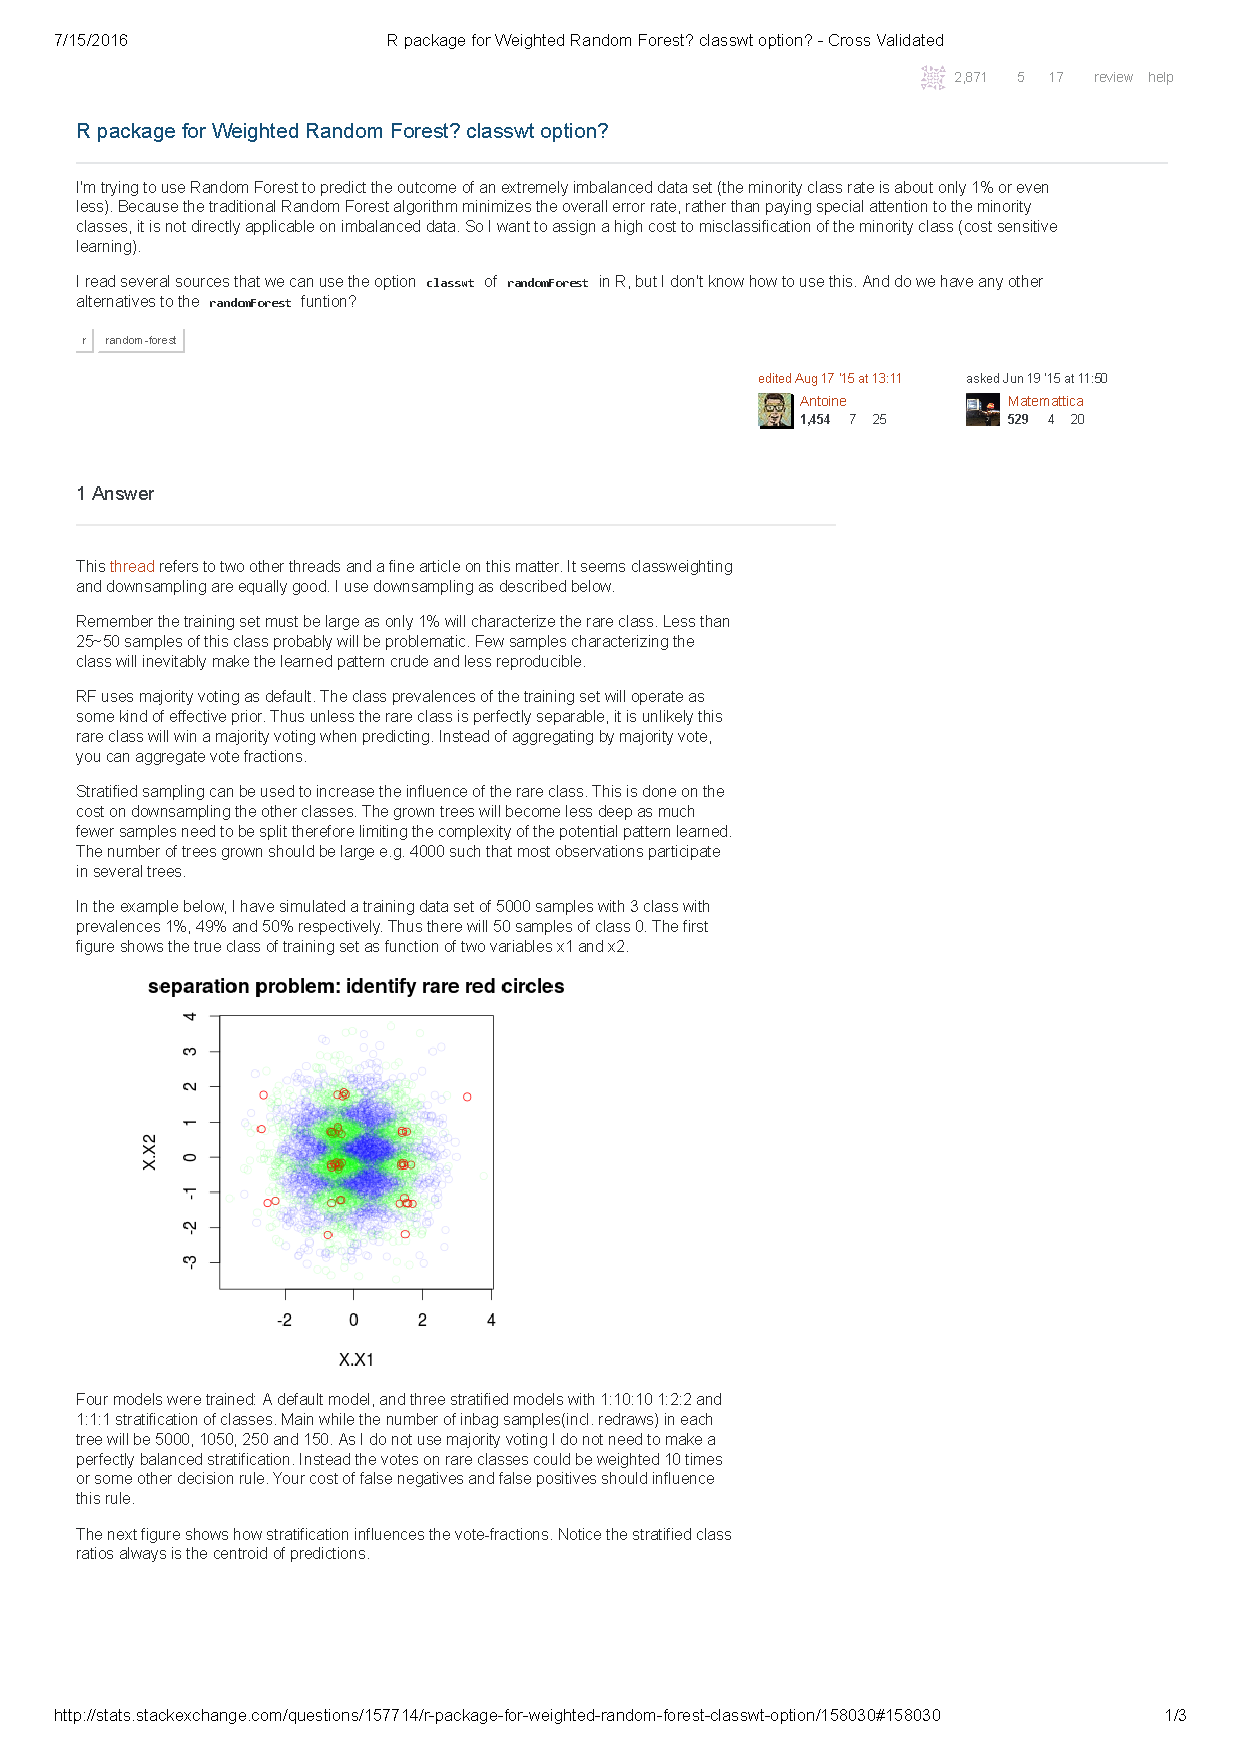
\includepdf[pages={1-},scale=0.90,pagecommand={\pagestyle{myruled}}]{cross_validated_posts/CV1_classwt.pdf}


\subsection{Random forest and outliers I: Outlier Islands}
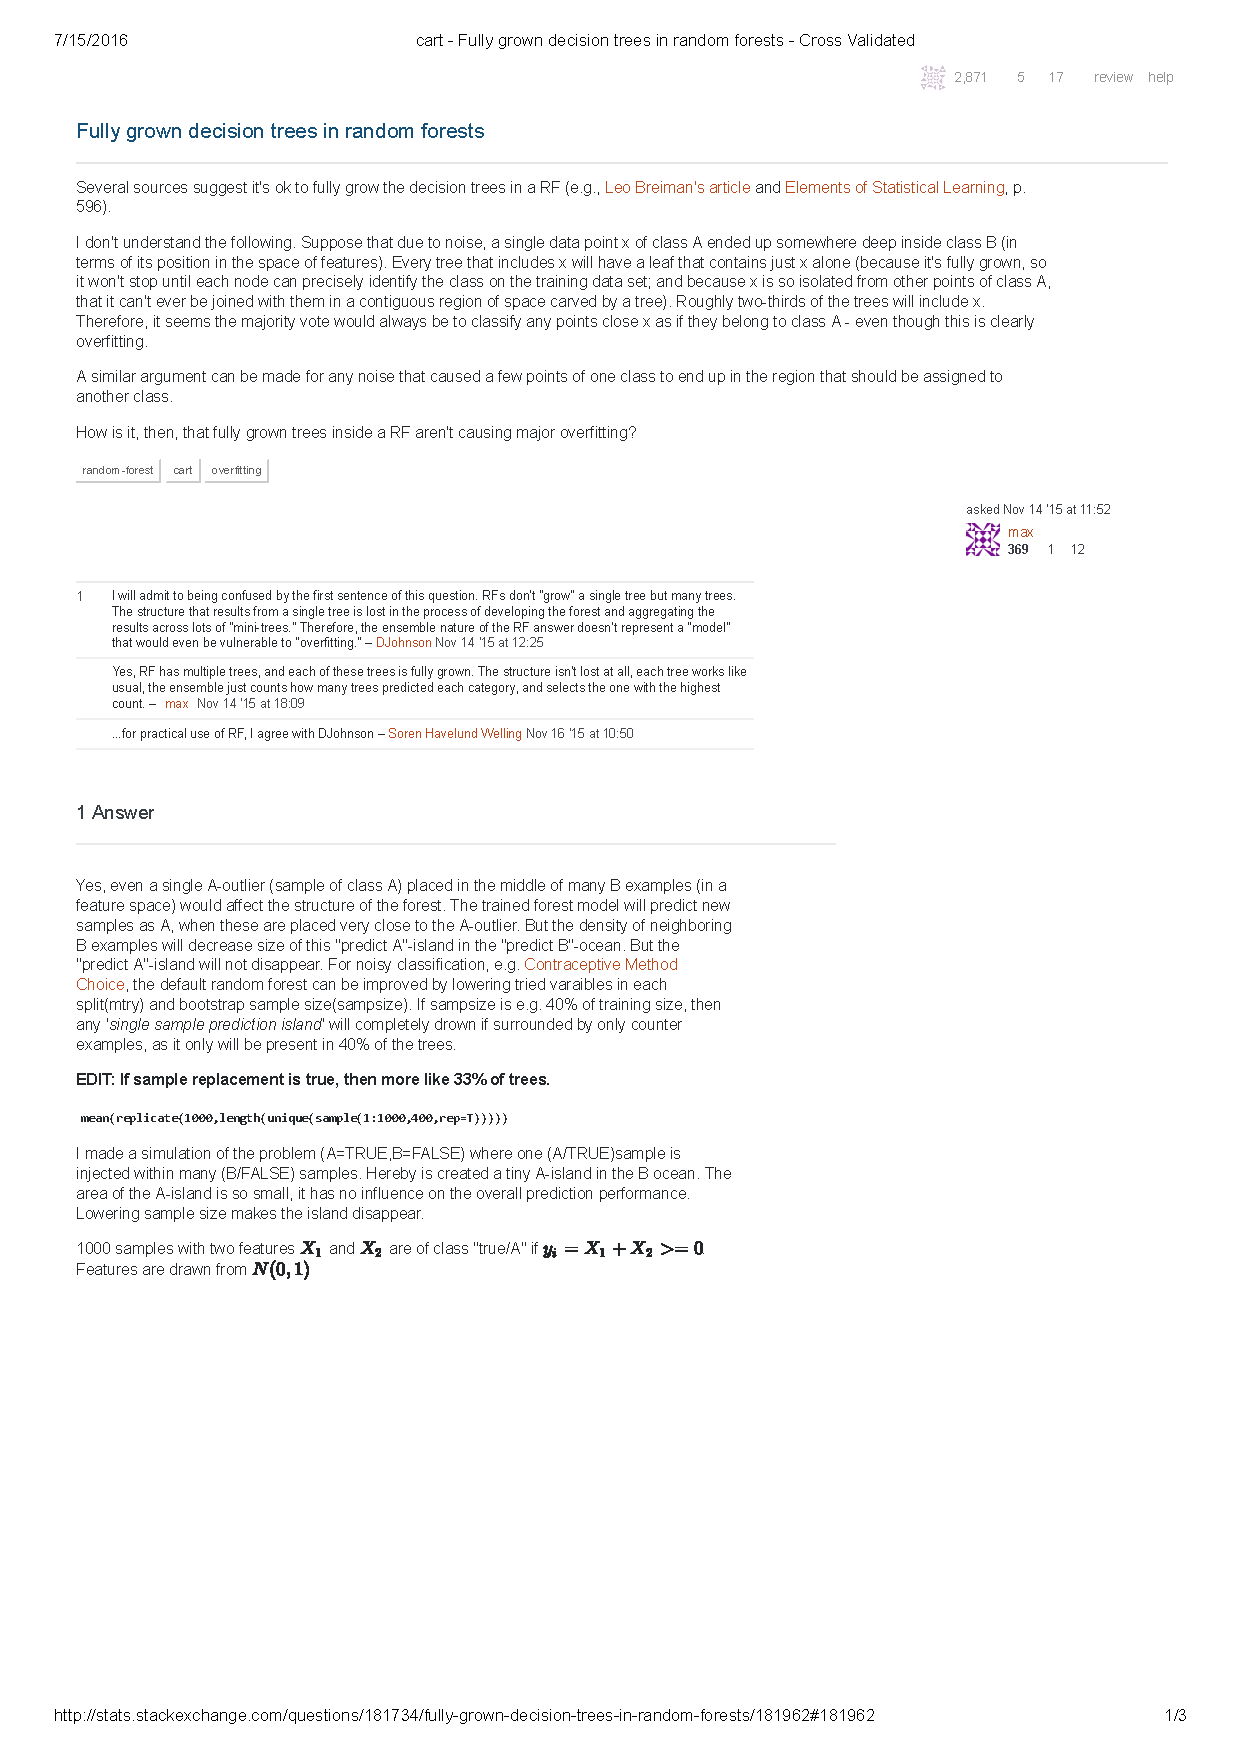
\includepdf[pages={1-},scale=0.90,pagecommand={\pagestyle{myruled}}]{cross_validated_posts/CV2_fullygrown.pdf}


\subsection{Random forest and outliers II: Robustness}
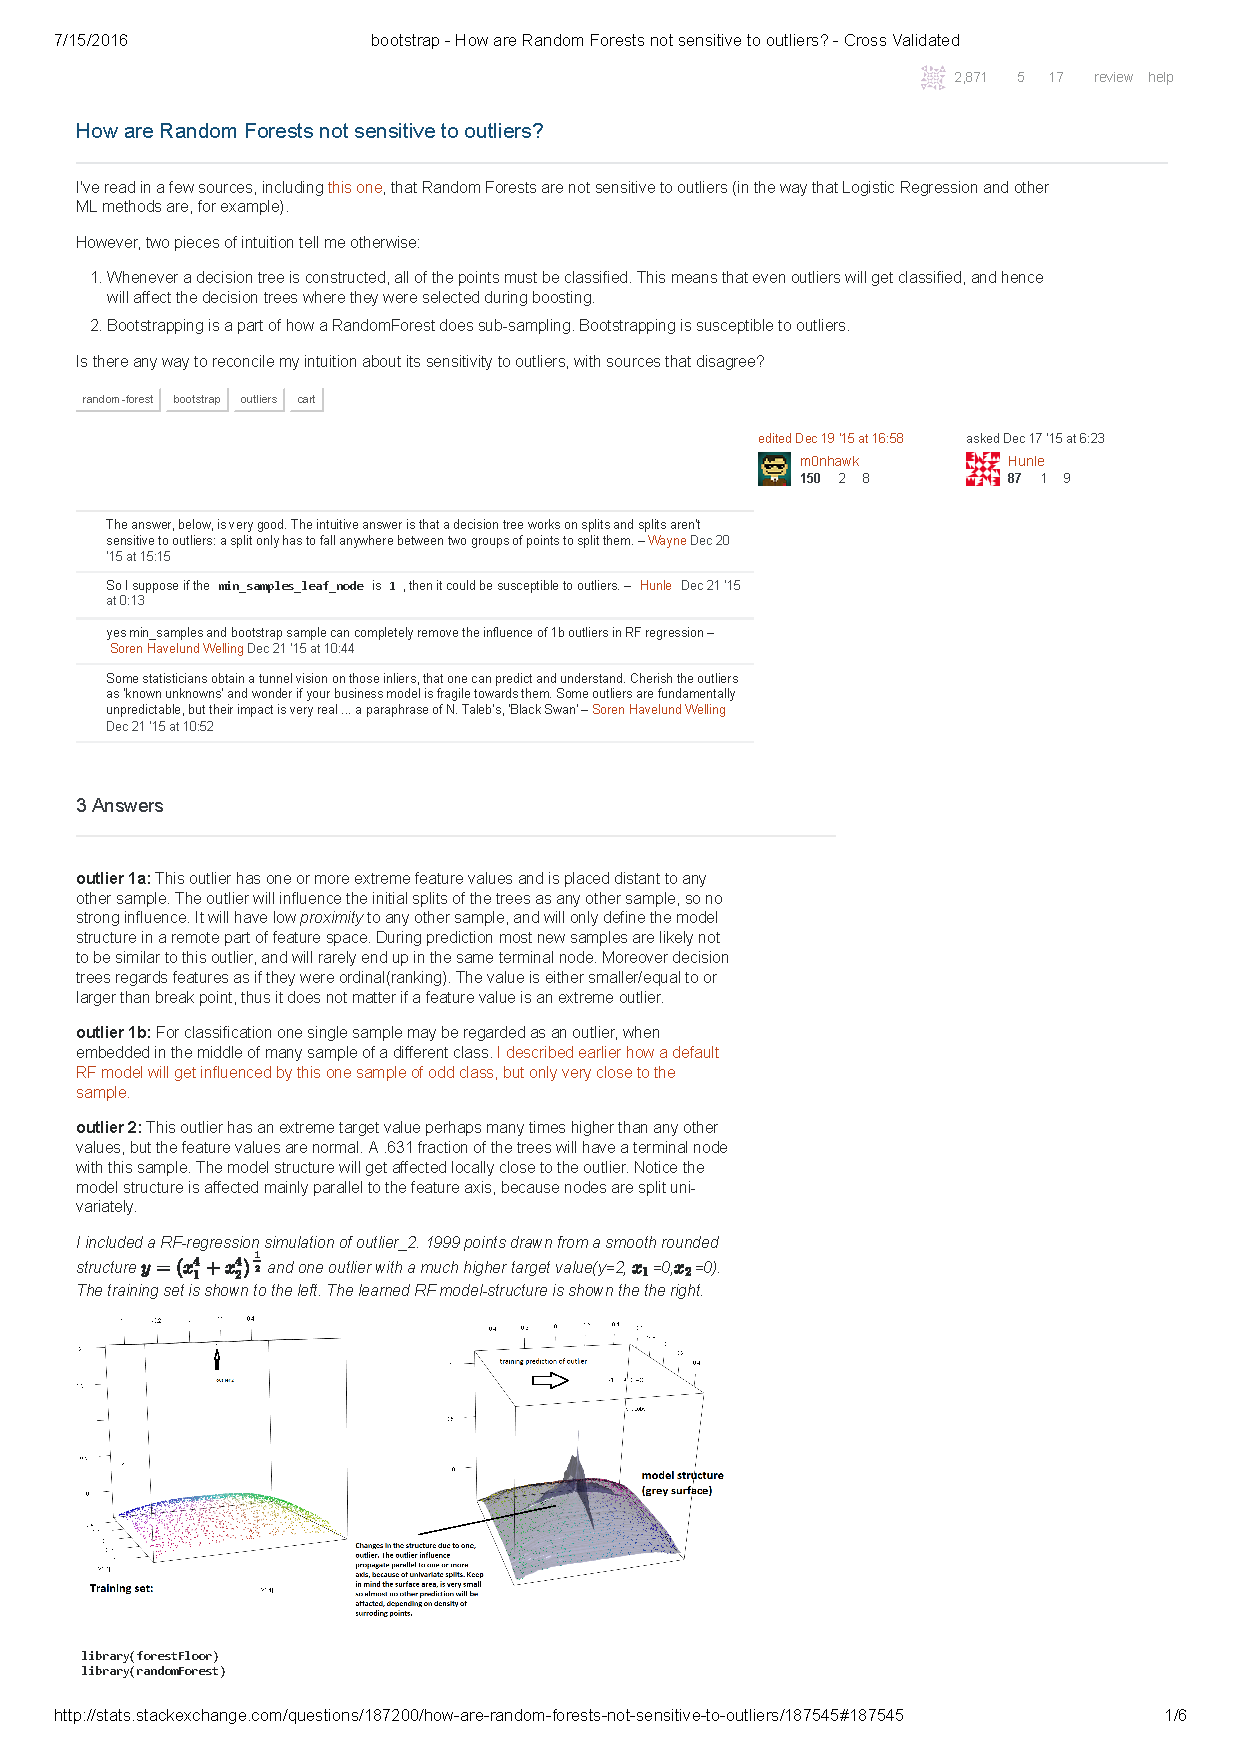
\includepdf[pages={1-},scale=0.90,pagecommand={\pagestyle{myruled}}]{cross_validated_posts/CV3_sensitiveOutliers.pdf}

\subsection{Simple check that random forest can fit interactions}
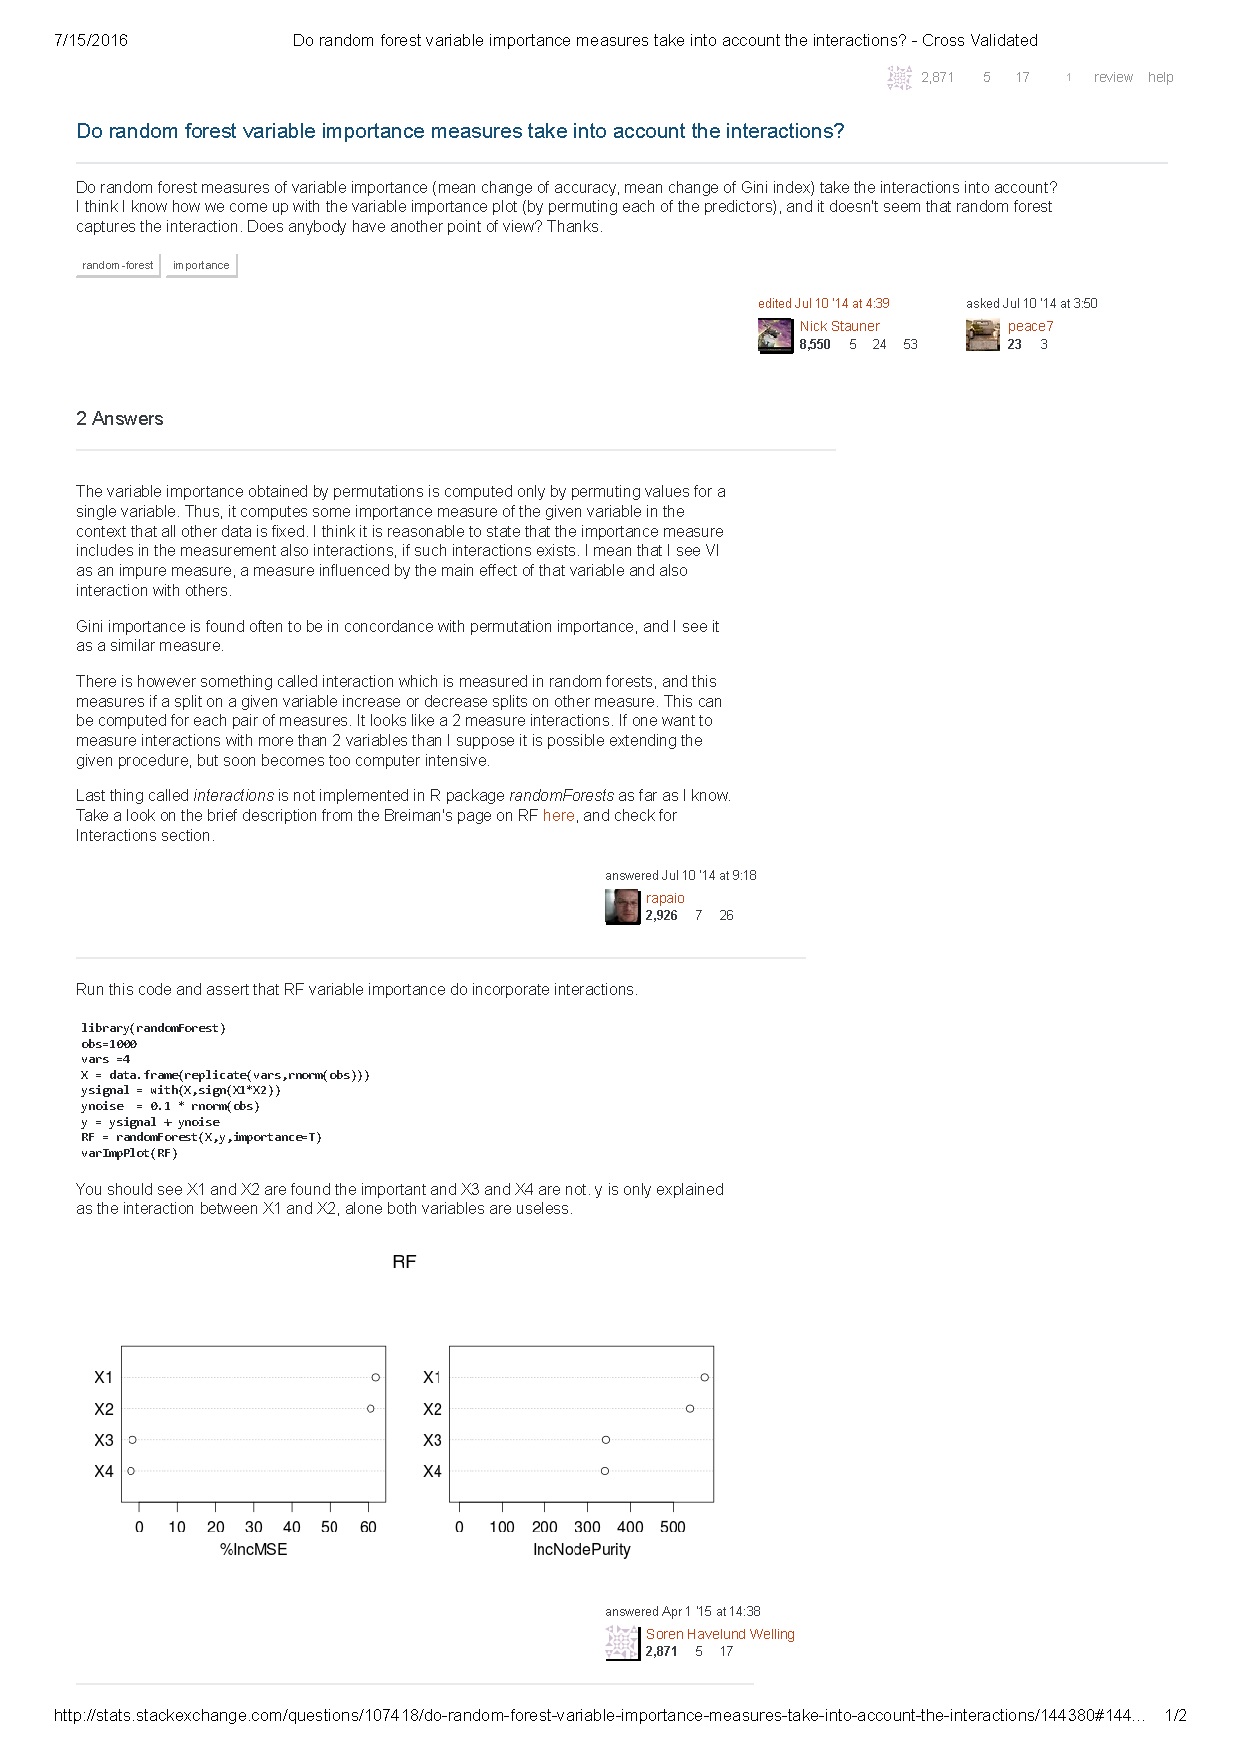
\includepdf[pages={1-},scale=0.90,pagecommand={\pagestyle{myruled}}]{cross_validated_posts/CV4_assertInteraction.pdf}

\subsection{Interpolation with RF and SVM is near}
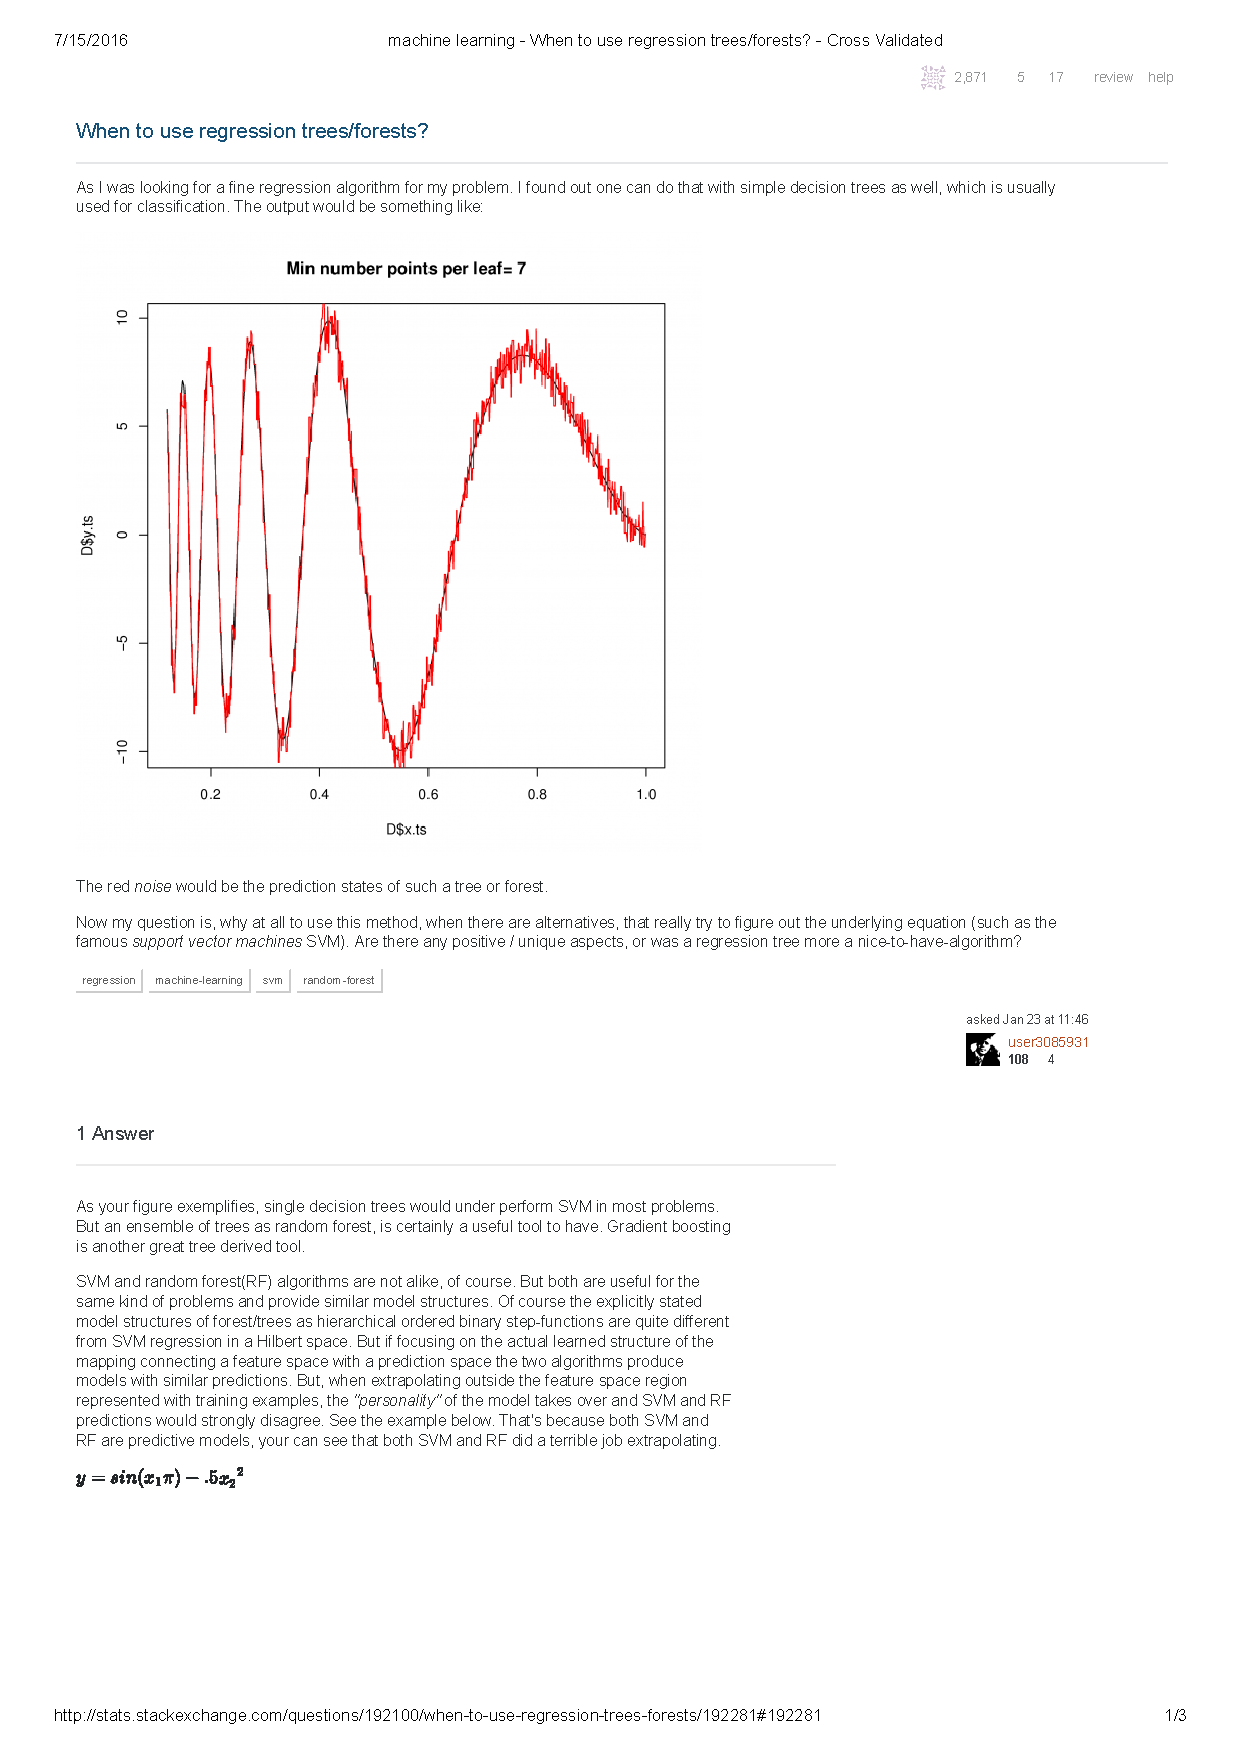
\includepdf[pages={1-},scale=0.90,pagecommand={\pagestyle{myruled}}]{cross_validated_posts/CV5_SVM_RF_same_same.pdf}

\subsection{How does CART break ties}
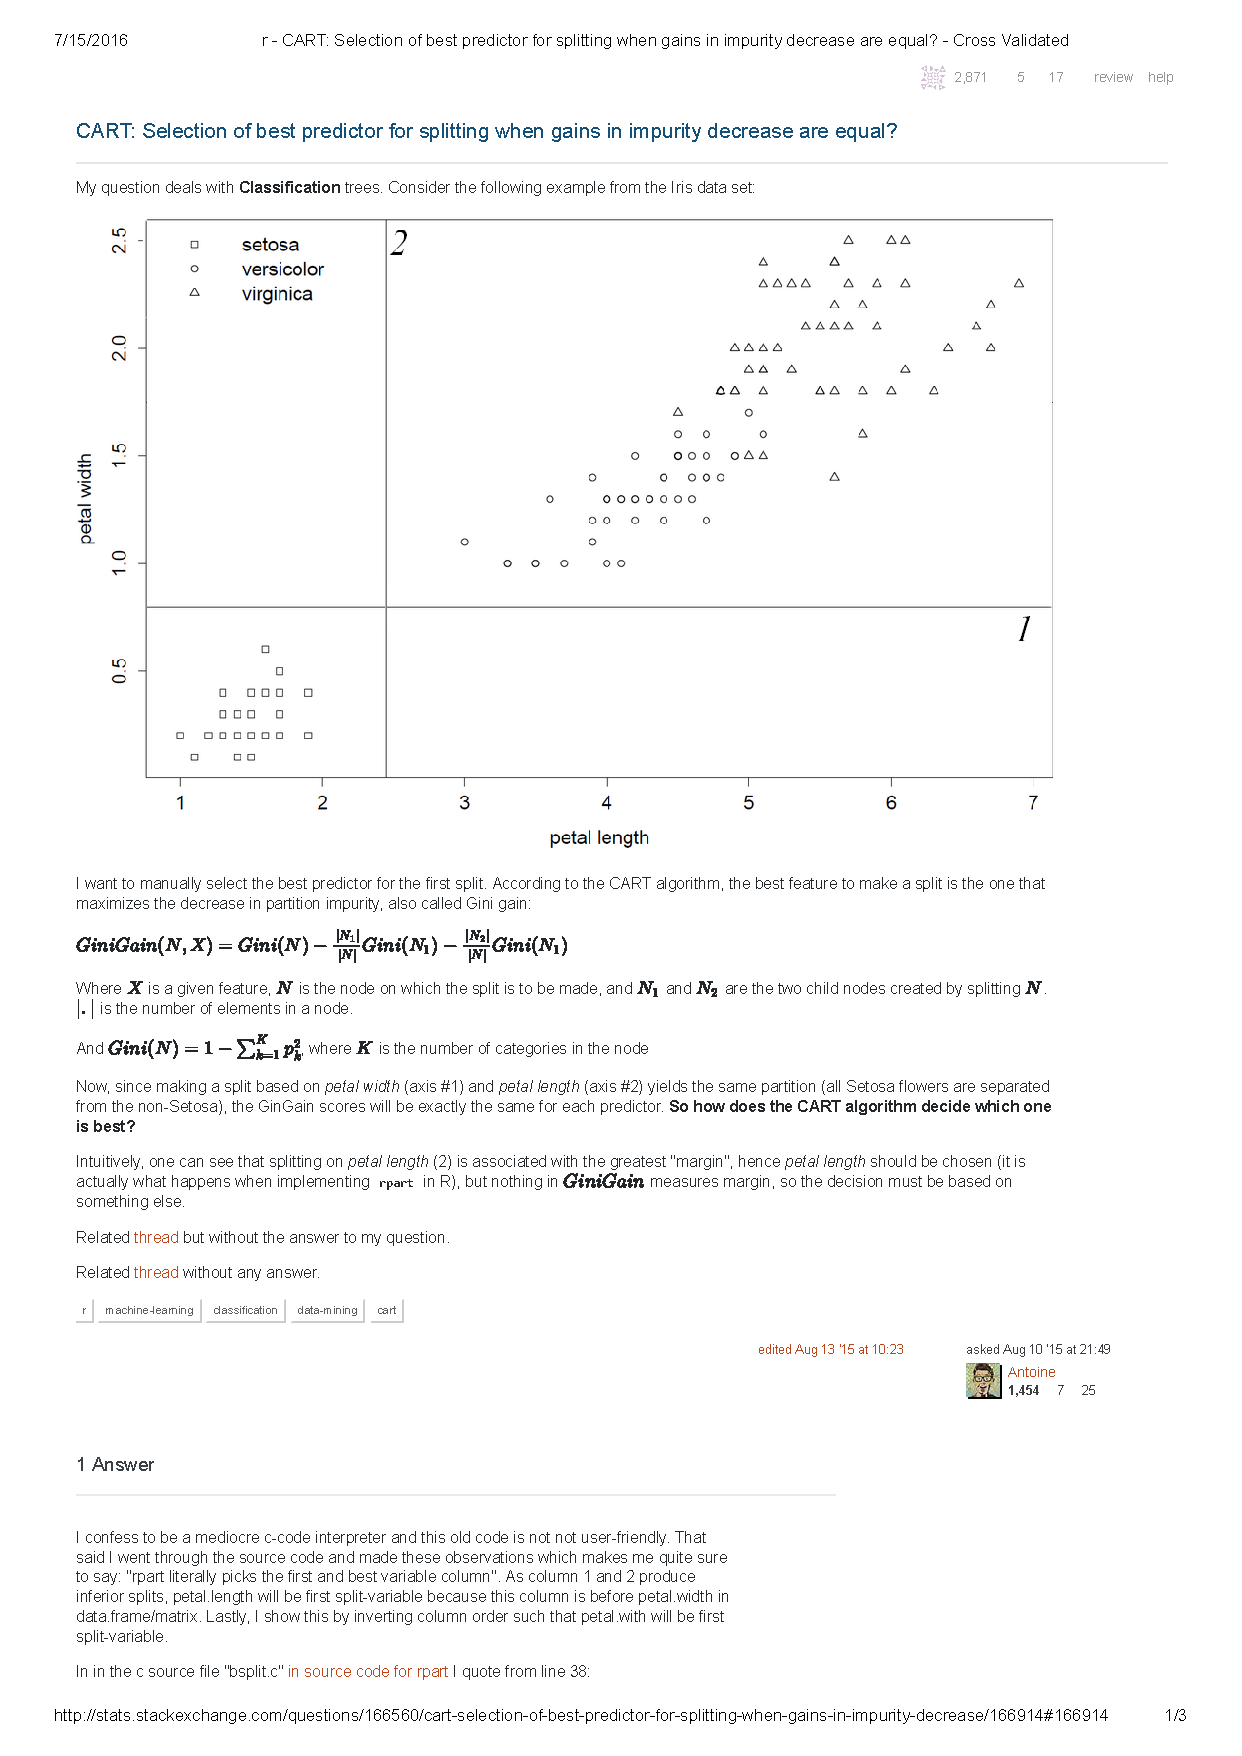
\includepdf[pages={1-},scale=0.90,pagecommand={\pagestyle{myruled}}]{cross_validated_posts/CV6_CARTtiebreak.pdf}

\subsection{Variable importance for other models than random forest}
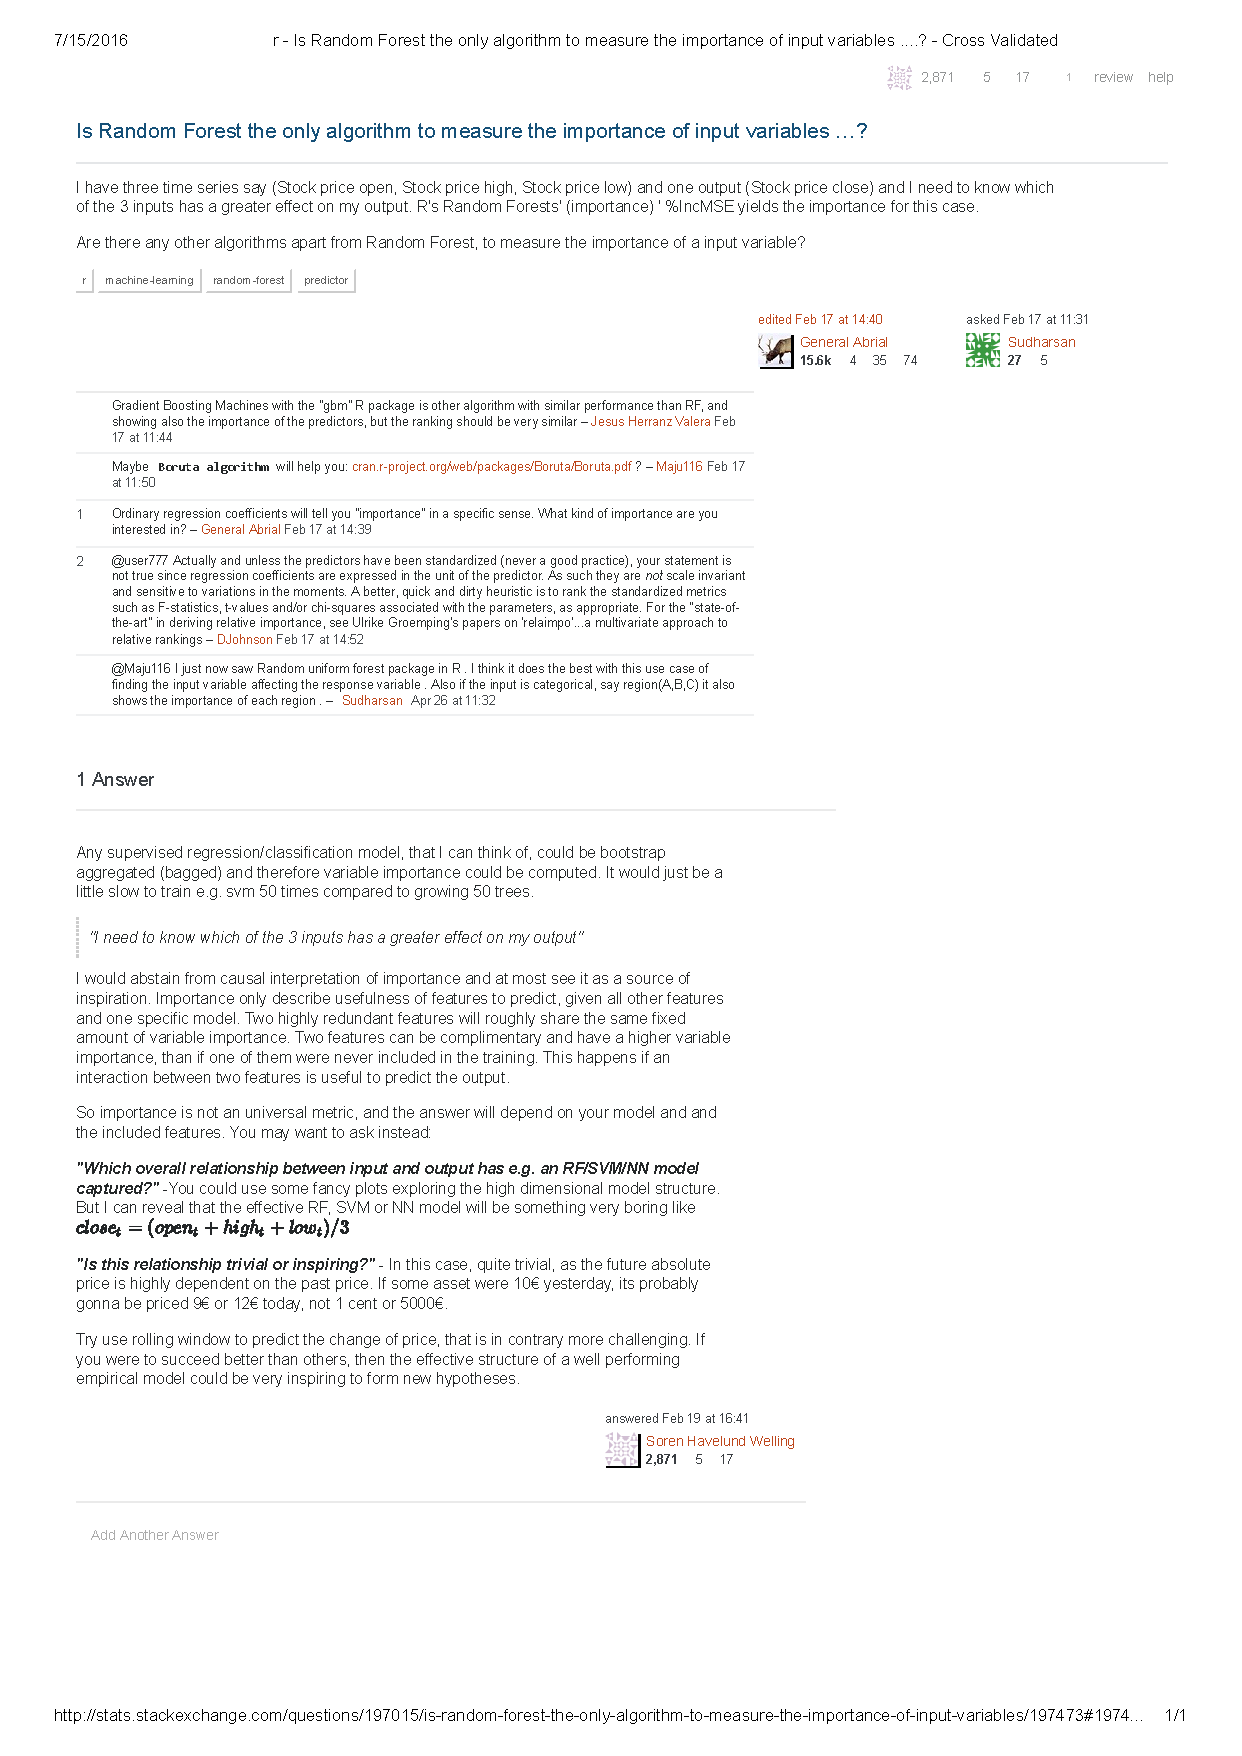
\includepdf[pages={1-},scale=0.90,pagecommand={\pagestyle{myruled}}]{cross_validated_posts/CV7_VIbeyondRF.pdf}

\subsection{How to combine multiple models in a bootstrap aggregated ensembles}
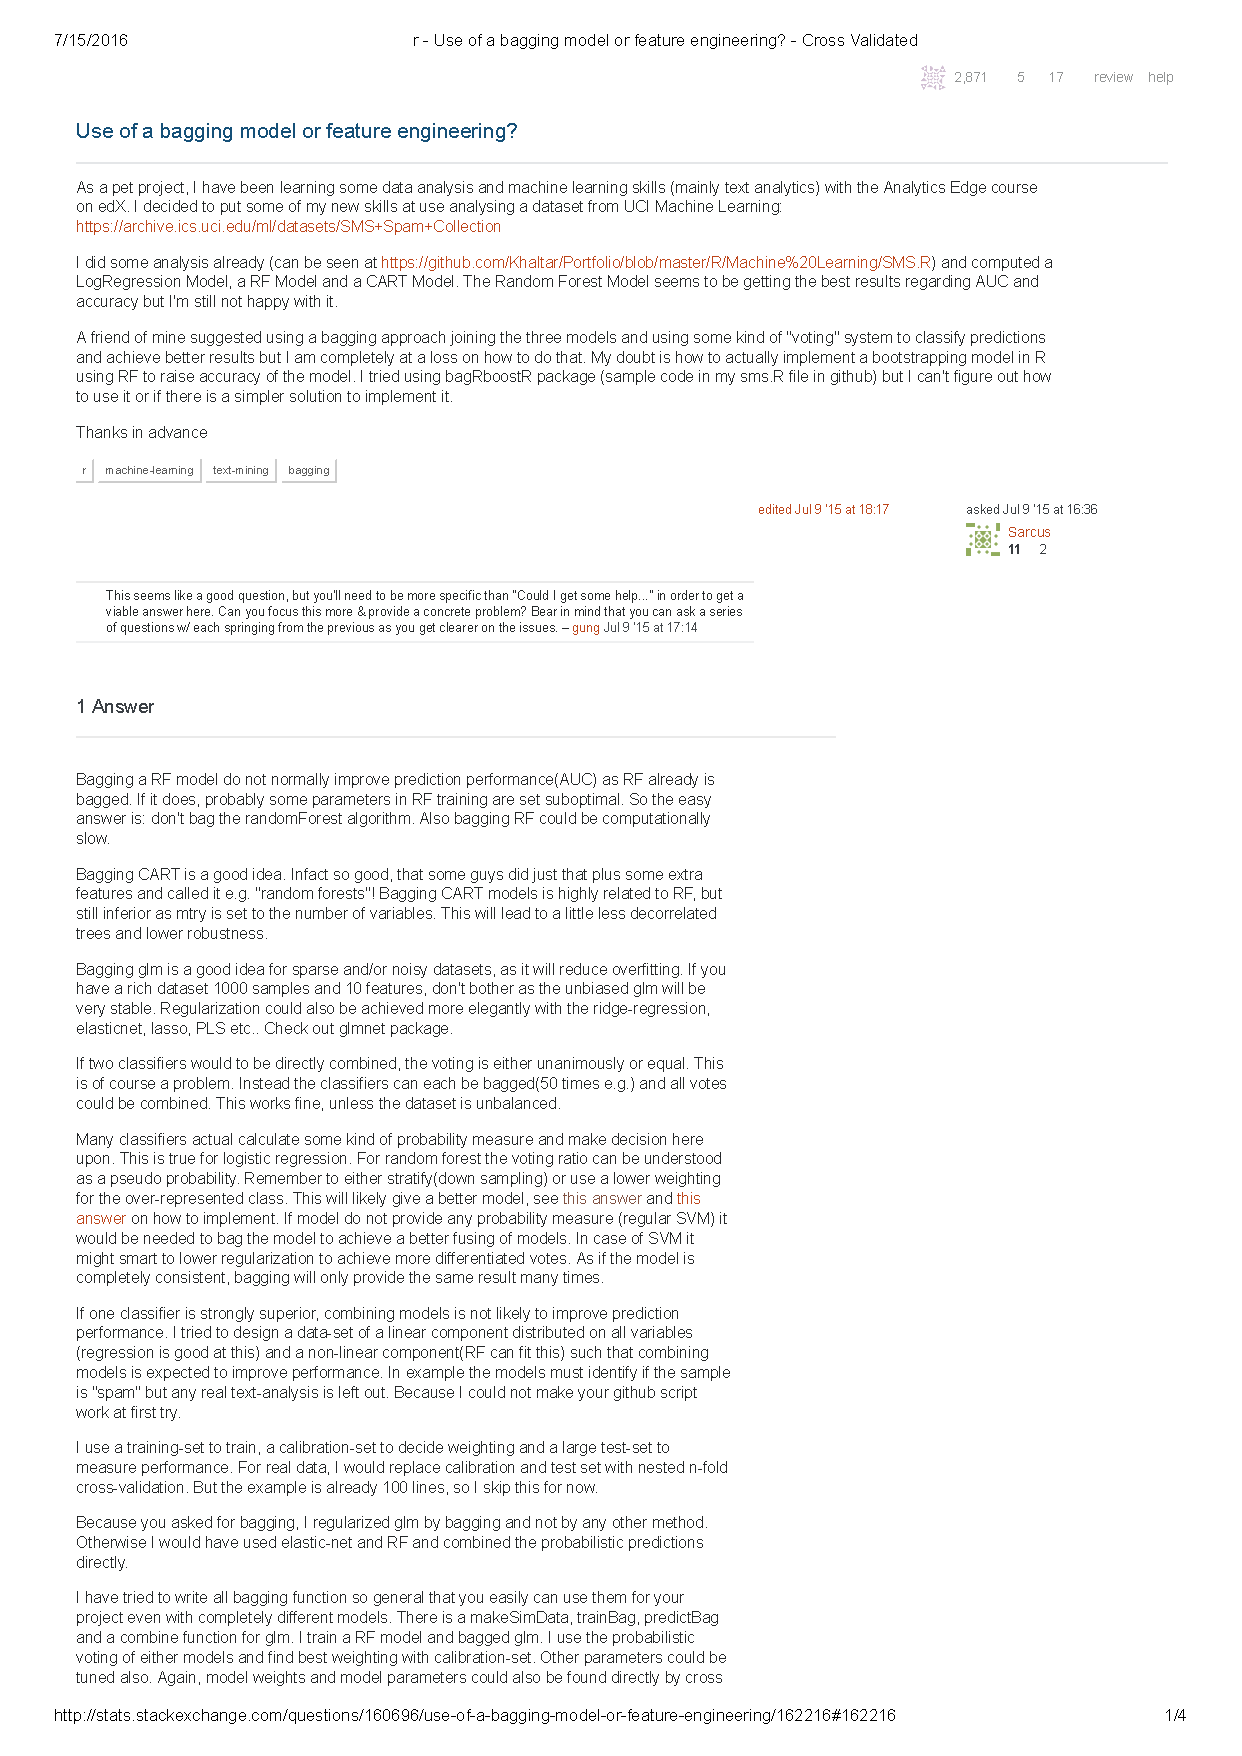
\includepdf[pages={1-},scale=0.90,pagecommand={\pagestyle{myruled}}]{cross_validated_posts/CV8_combineBagging}

\subsection{Bootstrapping process of random forest: Sampling proability as function of hyperparameters.}
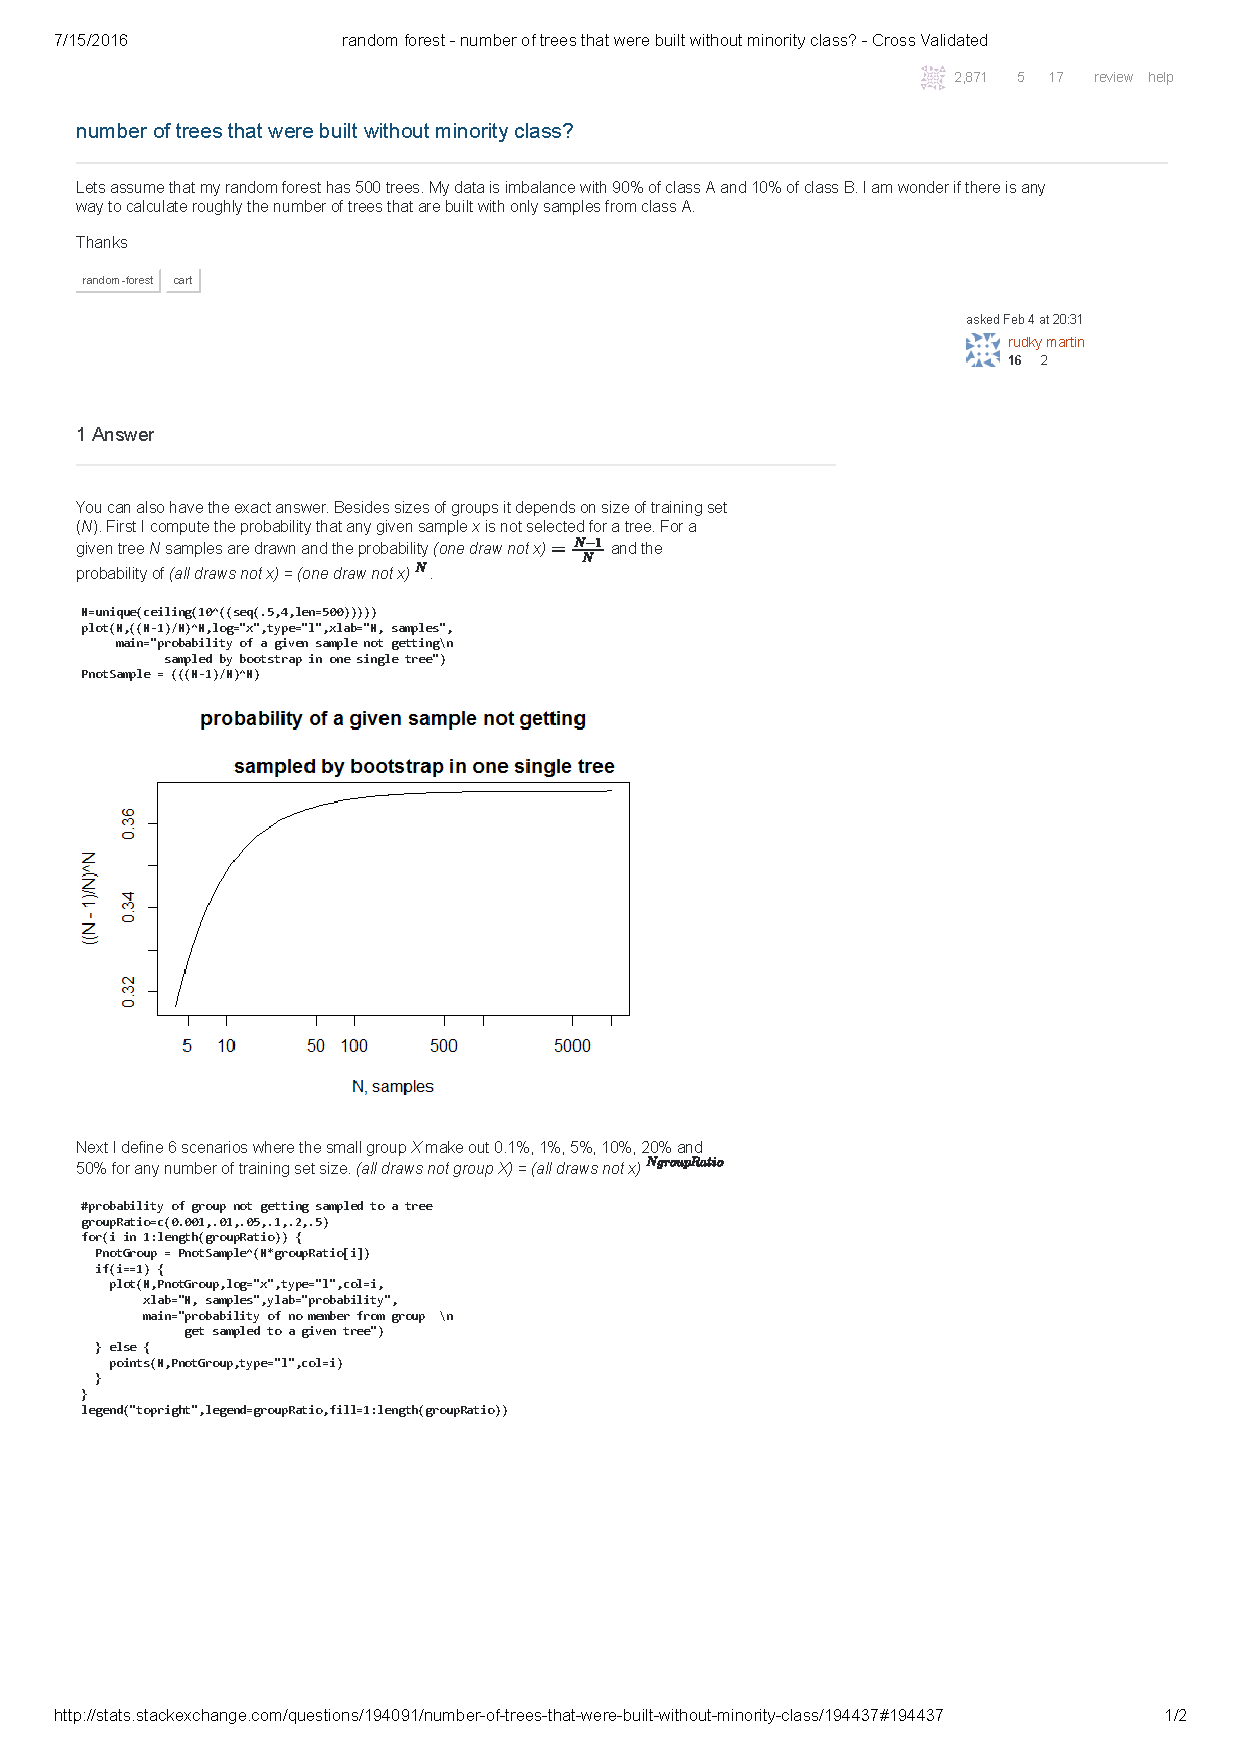
\includepdf[pages={1-},scale=0.90,pagecommand={\pagestyle{myruled}}]{cross_validated_posts/CV9_RFsampling}

\subsection{Simple tutorial explaining when log tranforming prior to PCA is reasonable}
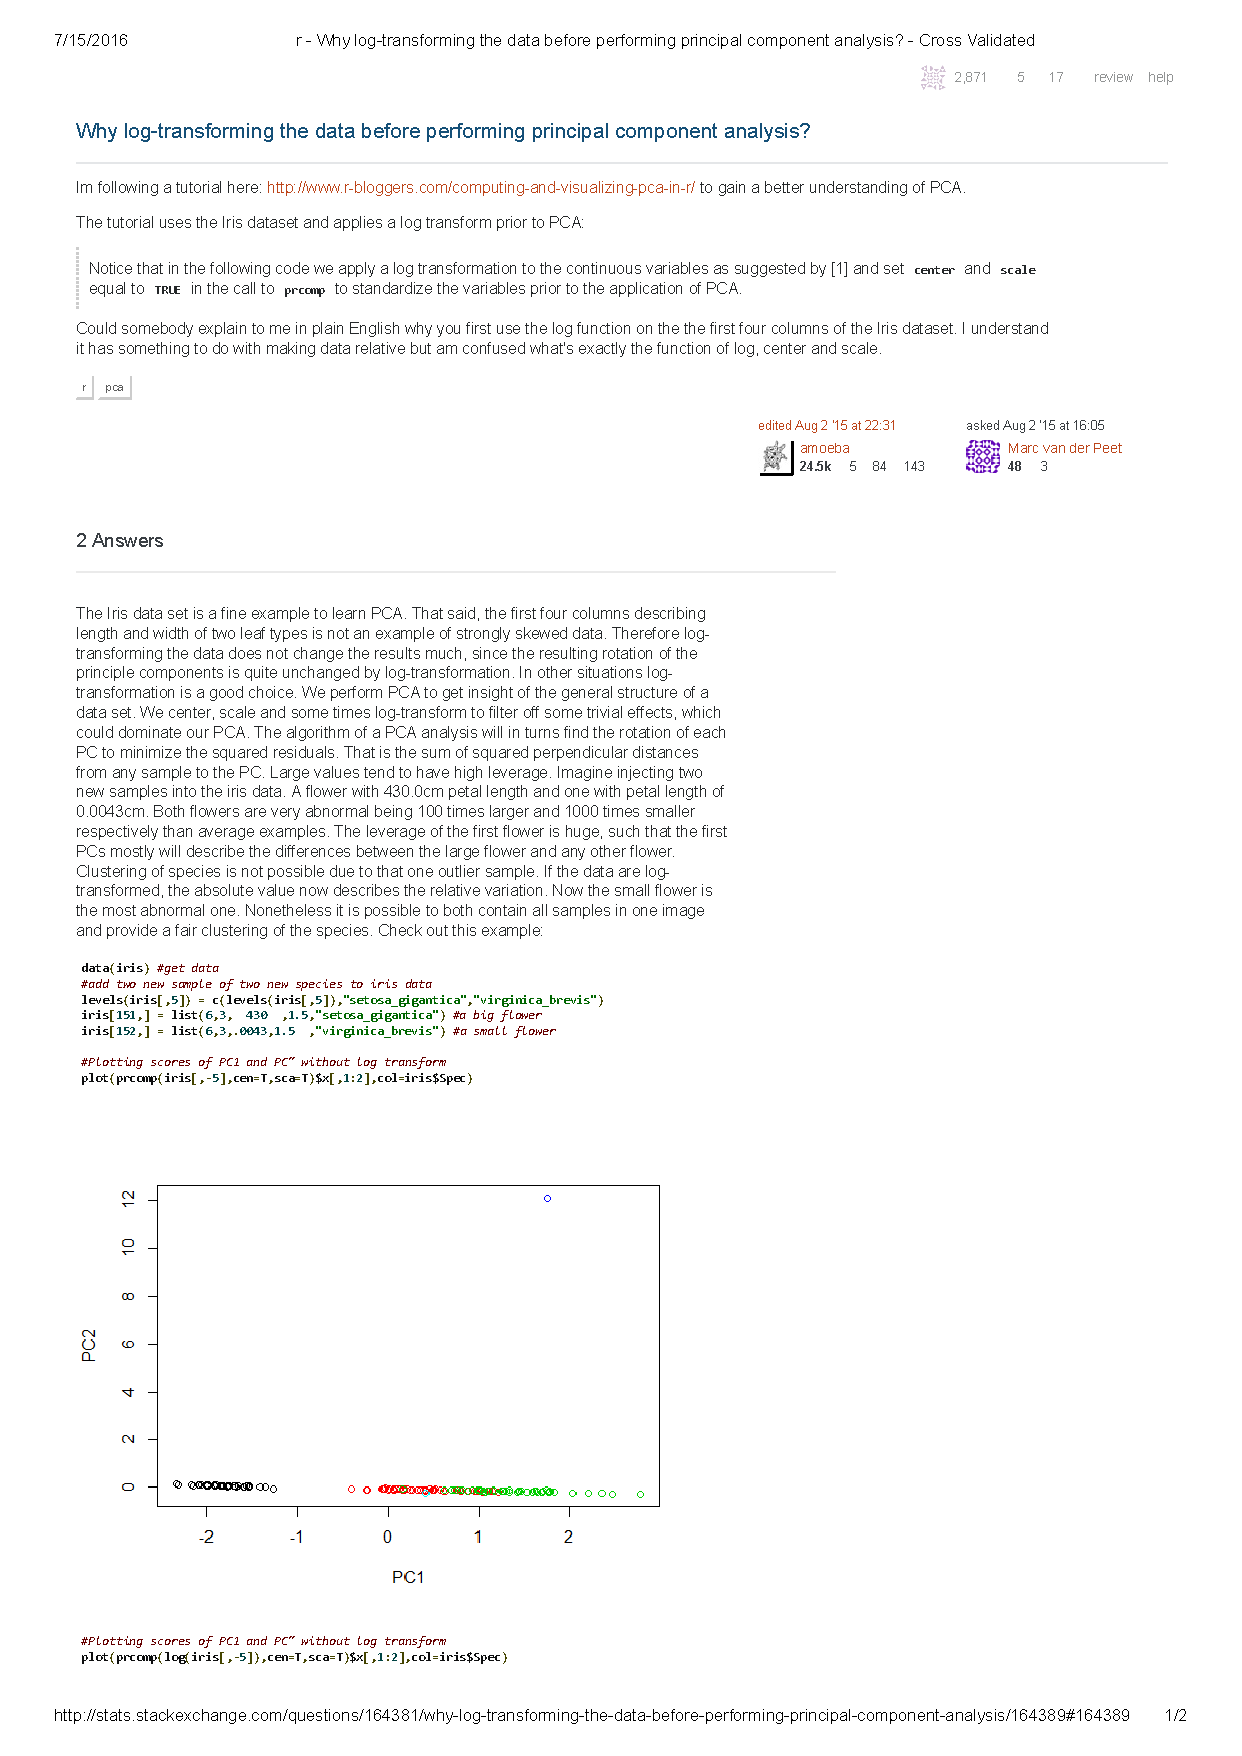
\includepdf[pages={1-},scale=0.90,pagecommand={\pagestyle{myruled}}]{cross_validated_posts/CV10_PCAlogTransform}




\section{Manual: R CRAN package forestFloor 1.9.5}

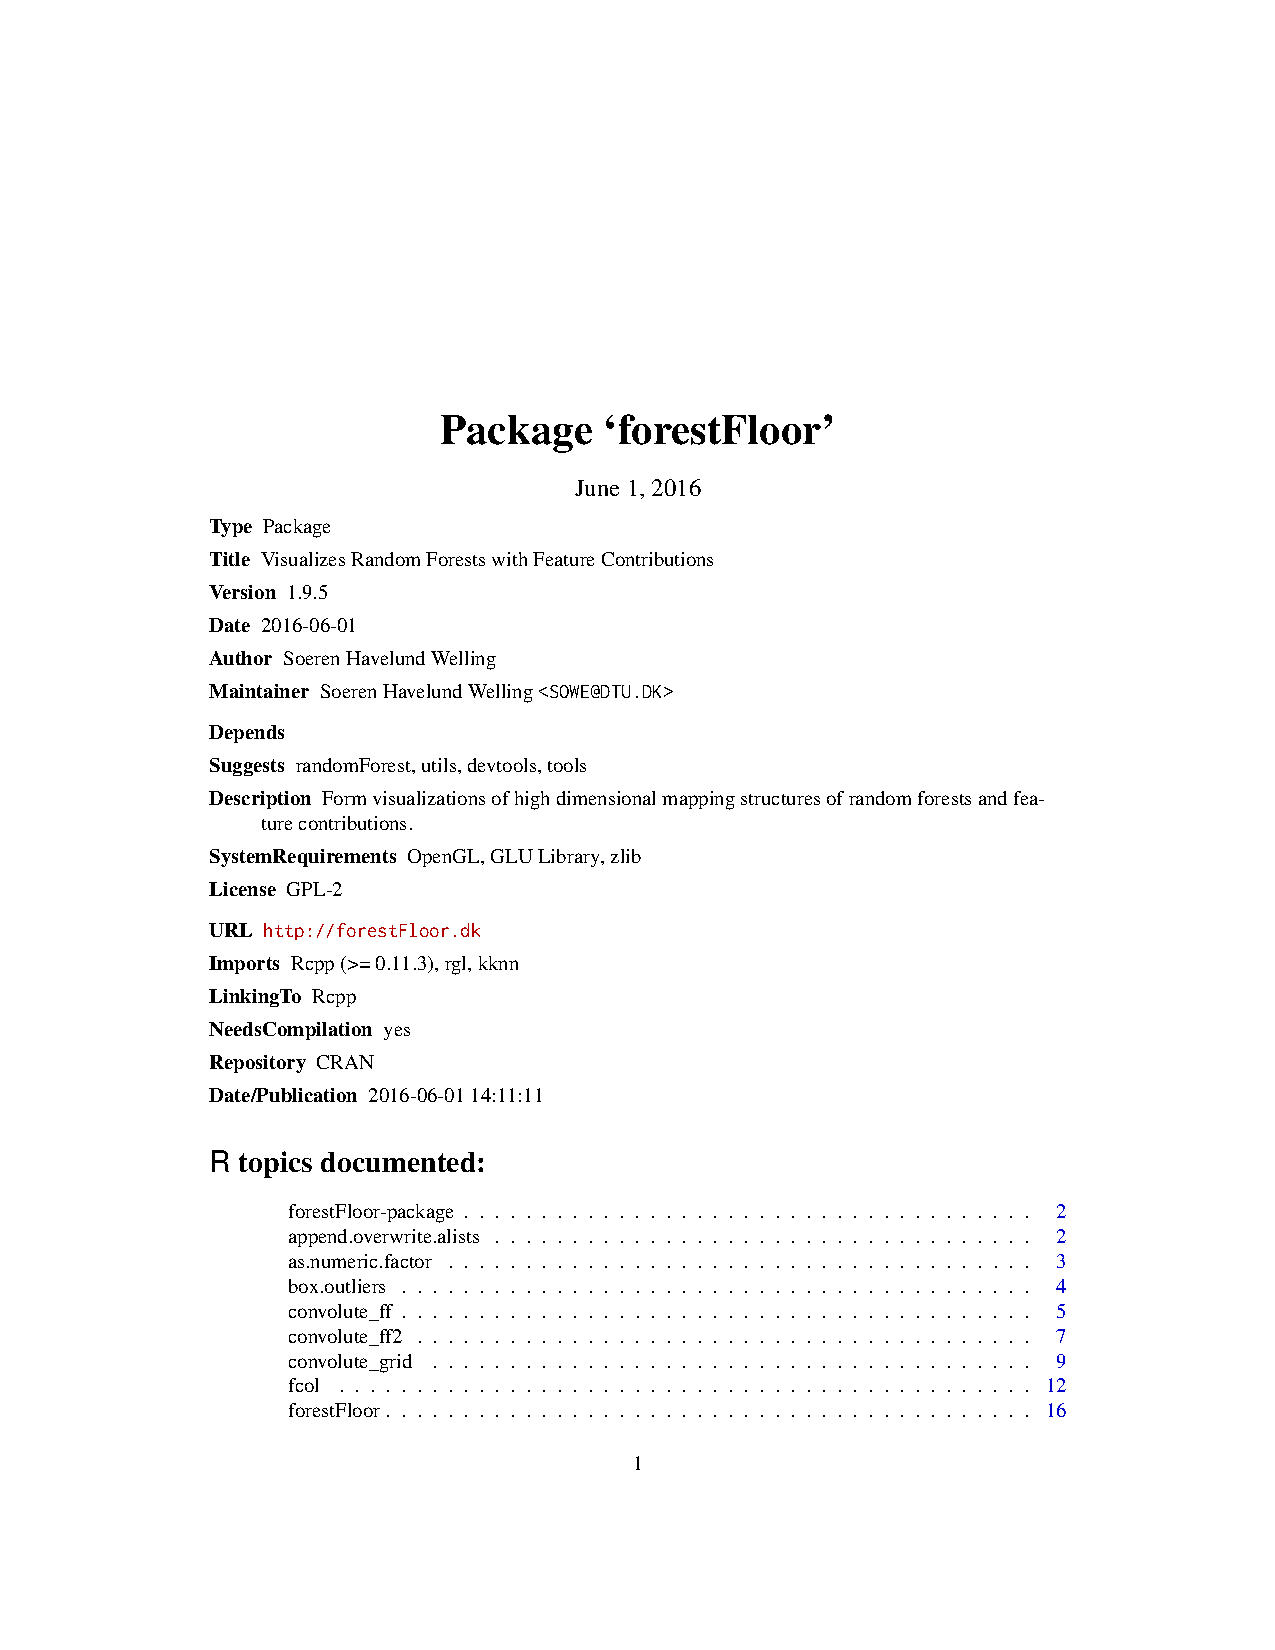
\includepdf[pages={1-},scale=0.90,pagecommand={\pagestyle{myruled}}]{appendices/forestFloorManual.pdf}

